\chapter{Distribution-based Grammar Evolution of L-systems}

\section{Overview}
To generate L-system plants that are aesthetically pleasing, varied and could be used to create offspring similar to its parents (\textbf{RQ0}), an algorithm called Distribution-based Grammar Evolution of L-systems (DGEL) was developed.

The DGEL name consists of two parts that are essential to solve the three sub research questions: \textit{Grammar Evolution (GE)} and \textit{Distribution-based}.
It uses GE to evolve L-system plants because it allows the algorithm to use well-researched techniques for modifying or combining genes into new L-systems (\textbf{RQ1}). 
As part of the GE process, there is a fitness function that evaluates how aesthetically pleasing a plant is, thus pushing the evolution towards aesthetically pleasing plants (\textbf{RQ2}).
It is distribution-based, meaning that different probability distributions for the L-system grammar can be used to generated varied plants (\textbf{RQ3}).

\begin{figure}
    \centering
    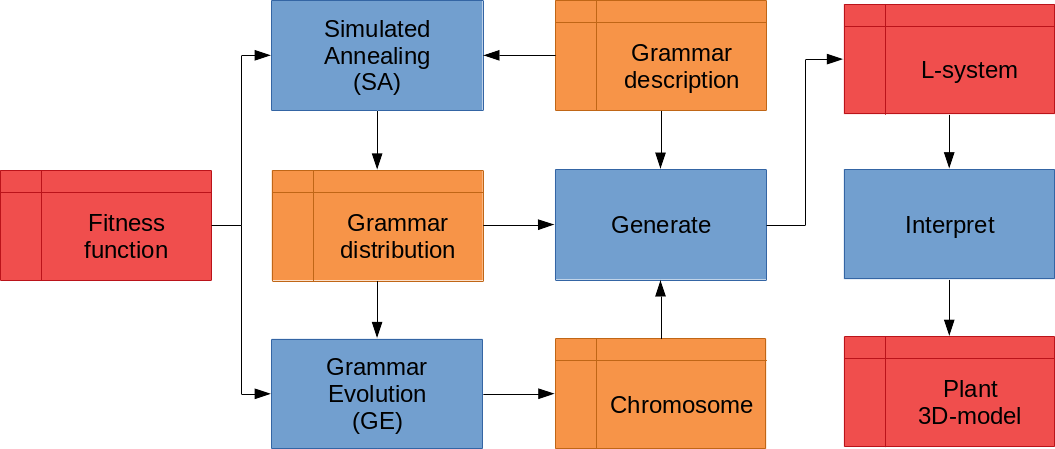
\includegraphics[width=1.0\textwidth]{figures/dgel}
    \caption[Overview of DGEL]{Overview of DGEL. Blue boxes represent processes. Red and orange boxes represent models. Orange boxes represent the models that define a unique L-system.}
    \label{fig:dgel}
\end{figure}

Figure~\ref{fig:dgel} illustrates the processes and models of the DGEL algorithm.
A plant 3D model is interpreted from an L-system.
The L-system is generated by a chromosome using a grammar distribution for a grammar description.
These three models: the grammar description, grammar distribution and the chromosome, together define the L-system.
All L-systems generated using the same grammar description, grammar distribution and chromosome will result in the exact same L-system, which also will be interpreted into the exact same plant 3D model.
GE is used to generated a good chromosome based on the grammar description, grammar distribution and a fitness function.
The grammar distribution is generated by Simulated Annealing (SA) based on the grammar description and a fitness function.
The fitness function models how aesthetically pleasing a plant is by assigning it score in range $[0, 1]$, where 0 is the worst, and 1 is the best.

\section{Representing an L-system with Grammar}
\label{sec:grammar}
As described, the L-systems in DGEL are represented by a chromosome, a grammar description and a grammar distribution.
If we assume a uniform grammar distribution, only a chromosome and a grammar description is required.

The grammar description, represented in a format such as the Backus Naur Form (BNF), describes the syntax of the L-system.
For example, it may describe that an L-system consists of a number of rules, each with a predecessor and successor, where a predecessor contains one character, etc.
The chromosome describes the choices to be made in the grammar description, for example how many rules there are, or which character the predecessor contains.
These choices are what creates the variations in the L-systems.
If there were no choices, there would only exist one single L-system.

This method of representing the L-systems was based on Beaumont and Stepneys's work on applying GE to plant L-systems~\cite{2009Beaumont}, in addition to Ortega et al.'s work on applying it to fractal L-systems~\cite{2003Ortega}, and Ryan et al.'s introduction of GE~\cite{1998Ryan}.

While Ortega et al.\ and Beaumont and Stepney make assumptions about the grammar to significantly simplify it and reduce the search space~\cite{2003Ortega, 2009Beaumont}, the DGEL method uses a grammar that covers the largest search space reasonably possible.
To make the search space reasonable, there still have to be some limits.
The number of productions, string length, and number of characters for a variable were limited to a maximum of 20.
A higher number did not seem reasonable as no L-systems in the literature reviewed used larger numbers, and the search times for higher numbers started to become unreasonable long.

Additionally, to limit the complexity of L-systems, complex features such as leaves, flowers, branch width and more were not included.
Thus the grammar used can only produce the branches of a plant.
This is the most essential part of a plant, which can be expanded later by modifying only the grammar description.
Listing~\ref{lst:grammar} shows the actual grammar description used during the development and testing of the algorithm, while Listing~\ref{lst:grammar2} shows a grammar description that supports leaves and varying branch width.

\begin{lstlisting}[caption=ABNF grammar description used in DGEL, label=lst:grammar, float]
lsystem = axiom productions
axiom = string
productions = 1*20production
production = predecessor successor
predecessor = variable
successor = string
string = 1*20(symbol / stack)
stack = "[" string "]"
symbol = variable / operation
variable = %x41-55
operation = "+" / "-" / "^" / "&" / ">" / "<"
\end{lstlisting}

\begin{lstlisting}[caption=ABNF grammar description supporting leaves and varying branch width, label=lst:grammar2, float]
lsystem = axiom productions
axiom = string
productions = 1*20production
production = predecessor successor
predecessor = variable
successor = string
string = 1*20(symbol / stack / leaf)
symbol = variable / operation
variable = %x41-55
operation = "+" / "-" / "^" / "&" / ">" / "<" / "!"
stack = "[" string "]"
leaf = "['{+f-f-f+|+f-f}]"
\end{lstlisting}

To be able to use different grammar distributions, the chromosome representation is a different from that of Ryan et al.\ where each gene is an unsigned 8-bit integer and the choice to be made is the alternative index by the gene modulo the number of alternatives~\cite{1998Ryan}.
Each gene is still represented by an unsigned integer, but it is 32-bit instead of 8-bit, and the interpretation of the integer is different.

A gene in the DGEL chromosome can be viewed as an index into the value range of the 32-bit integer.
This value range, from $0$ to $2^{32}$, can be viewed as a line with segments representing each alternative in a rule in the grammar.
In the case of a uniform distribution the segments would be equal in length, while for a different distribution the lengths will differ.
The value of each gene in the chromosome is randomly picked from a uniform distribution, thus making the actual distribution dependent on the grammar distribution.

Figure~\ref{fig:gene} illustrates an example of this process.
A choice is to be made between $C$, $D$, $E$ and $F$ in the rule $A \rightarrow C / D / E / F$.
A chromosome of length 4 containing 4, 3, 0 and 7 is used, and the next gene to be used in the chromosome is the second position, i.e.\ the value 3.
Each gene is a 3-bit unsigned integer, thus having 8 possible values in range $[0, 8)$.
Since there are four alternatives, and a uniform distribution is used, the 3-bit value range is split into four segments of 2 values.
The gene value 3 maps into the second segment, which maps to the second alternative in the rule, i.e.\ $D$.
This process would then continue with the next gene, 0, on the $D$ rule.

\begin{figure}
    \centering
    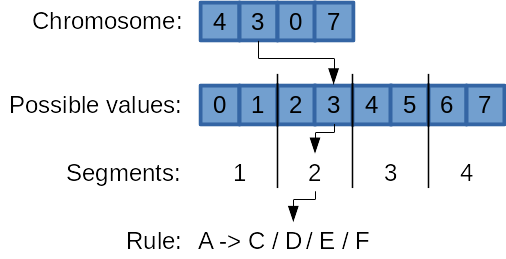
\includegraphics[width=0.8\textwidth]{figures/gene}
    \caption[Example grammar alternative selection from gene]{Example grammar alternative selection from gene. In the figure, the gene is a 3-bit integer, and thus has 8 possible values.}
    \label{fig:gene}
\end{figure}

\section{Using a Grammar Distribution to Limit Search Space}
In DGEL, grammar distributions are used for three reasons: to guide the GE to more efficiently find good plants, to guide GE to search in a space with certain types of plants, and to prevent infinite recursion.

The distribution is a set of weights per choice per rule per depth, as illustrated in Figure~\ref{fig:distribution}.
The depth is the current branching depth of the L-system, controlled by the bracket operators, and defined as the \textit{stack} rule in the grammar in Listing~\ref{lst:grammar}.

The example figure shows a case where a choice is to be made between the alternatives C, D, E and F in rule $A \rightarrow *(C / D / E / F)$.
There are two different choices in the rule: selecting the number of repetitions (indicated by the asterisk character, \textit{*}), and selecting the C/D/E/F alternative.
In the example, the depth is 0 (no branching), the rule is $A$ and the choice is the second.
This maps to the weight array: $[0.1, 0.4, 0.3, 0.2]$ which should be applied to the C/D/E/F choice.
Thus, $C$ has a 10\% chance of being selected, $D$ has 40\%, $E$ has 30\%, and $F$ has 20\%.
These weights are then used to define the segments in the gene, as described in Section~\ref{sec:grammar}.

\begin{figure}
    \centering
    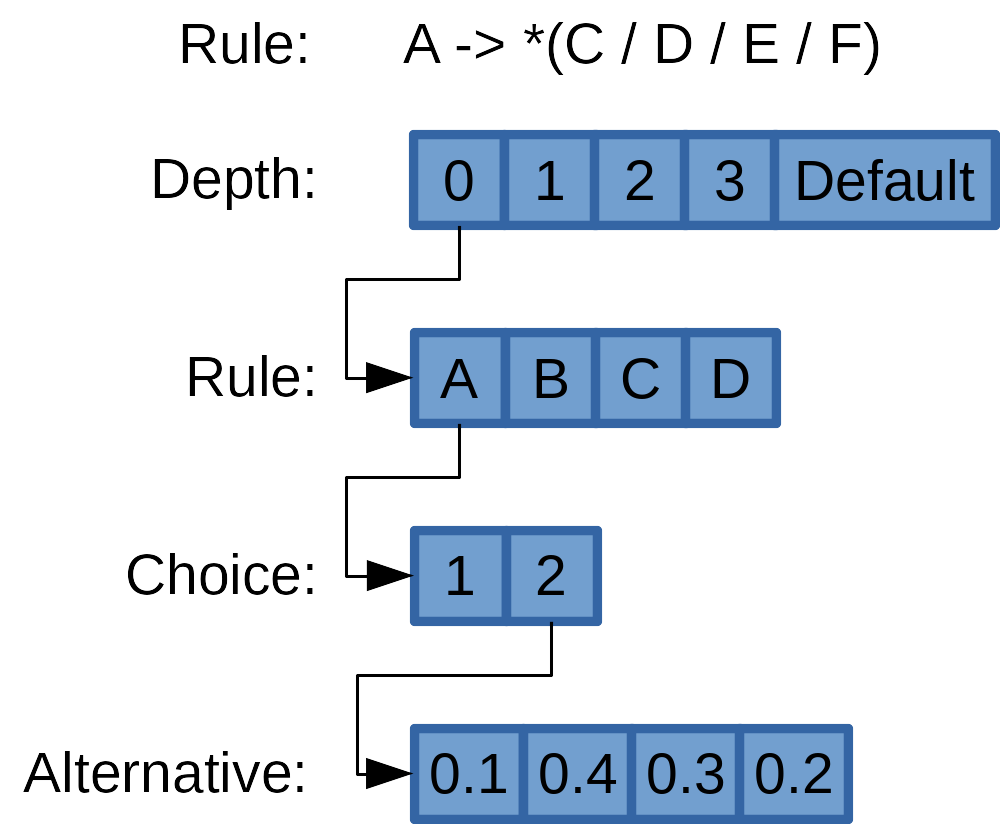
\includegraphics[width=0.6\textwidth]{figures/distribution}
    \caption[Example grammar distribution]{Example grammar distribution applied to the second choice of rule $A$ at depth 0.}
    \label{fig:distribution}
\end{figure}

By using a specialized distribution, rather than a uniform distribution, the generator may be targeted at specialized L-systems, or just have a higher average fitness score for the generated plants.
For example, the distribution may focus more on producing the \textit{F} character which is used for drawing the branches.
Or it may be focused on the \textit{stack} rule that produces branching points.
This may in turn increase the rate of produced plants that have long or many branches.

In addition to the distribution weights shown in Figure~\ref{fig:distribution}, there is a default distribution that will be used if there does not exist a mapping for a rule and choice at a specific depth.
This can be used to prevent infinite recursion with the \textit{stack} rule.
For example, the distribution for the grammar in Listing~\ref{lst:grammar} may specify the weights $[0.5, 0.5]$ for the second choice (\textit{symbol / stack}) in the \textit{string} rule at depth 0, 1 and 2, such that there is an equal change to produce a string and a stack (branching point).
To prevent any further branchings, the weights $[1.0, 0.0]$ may be specified for the default distribution, causing it to not produce a stack at depth 3 or deeper.

To find specialized distributions to more efficiently generate good plants or generate different types of plants, the weights in the distribution need to be optimized.
As the distribution maps from depth, to rule, to choice, to alternative (weight), it is a four-dimensional parameter space to be optimized.
DGEL uses Simulated Annealing (SA) to perform the optimization, but other multi-dimensional parameter optimizers could just as well be used.

Specifically, DGEL implements the basic SA approach~\cite{2000Ozdamar}, as described by Onbaşoğlu and Özdamar~\cite{2001Onbasoglu}.
The only difference is that the initial solution is not initialized randomly, but initialized from a pre-optimized solution, such that it has a better starting point.
In the DGEL SA, the \textit{solution} is the distribution itself, filled with weights for each of the alternatives in each of the choices in each of the rules in a limited set of depths.

A neighbour solution is generated in the same manner as Onbaşoğlu and Özdamar describes~\cite{2001Onbasoglu}: selecting one single random weight and either increasing or decreasing the weight randomly, bounded to the range $[0.0, 1.0]$ in the case of DGEL.
A key difference is that since these are \textit{weights}, the remaining weights in the same set of weights have to be modified such that the sum of all of the weights equal 1.
If the sum of the remaining weights is greater than 0, they can be scaled by a normalization factor, calculated by $\frac{(1 - w)}{(1 - w_0)}$, where $w$ is the new value of the modified weight, and $w_0$ is the old value of the modified weight.
If the sum of the remaining weights is exactly 0, scaling the weights will not work, as they would remain 0.
The alternative solution is to divide the ``remaining weight'' over the remaining weights.
This is done by setting the remaining weights to $\frac{(1 - w)}{(n - 1)}$, where $w$ is the new value of the modified weight, and $n$ is the number of weights.

Accepting a neighbour solution also follows the same approach as Onbaşoğlu and Özdamar describes~\cite{2001Onbasoglu}.
To do this, an $f(x)$, where $x$ is a grammar distribution, has to be defined.
The performance of a grammar distribution can not directly be measured, but it can be estimated by measuring the average performance of the L-systems it generates.
As the performance of the L-systems generated may vary by a big degree, the average performance is only accepted after a specified amount of L-systems have been generated, and the standard error of the performance is below a threshold value.

\section{Using Grammar Evolution to Search the Space}

\section{Using a Fitness Function to Evaluate Plants}